\documentclass{article}
\usepackage[utf8]{inputenc}
\usepackage[sfdefault,ultralight]{FiraSans} %% option 'sfdefault' activates Fira Sans as the default text font
\usepackage[T1]{fontenc}
\renewcommand*\oldstylenums[1]{{\firaoldstyle #1}}
\usepackage{appendix}
\usepackage{graphicx}
\usepackage{amsfonts}
\usepackage{amssymb}
\usepackage{xcolor}
\usepackage{fdsymbol}
\usepackage{wasysym}
\usepackage{multicol}
\usepackage{amsmath,seqsplit}
\usepackage{algorithm, algorithmic}
\usepackage{tcolorbox}
\usepackage{geometry}
 \geometry{
 a4paper,
 right=20mm,
 left=25mm,
 top=25mm,
 bottom=25mm,
 }
\usepackage{pgfplots}
\usepackage{hyperref}
\usepackage{tikz}
\newcommand\foo[2]{%
    \begin{minipage}{#1}
    \seqsplit{#2}
    \end{minipage}
}

\setlength{\columnsep}{1cm}
\setlength\parindent{0pt}

\usepackage{tkz-graph}

\hypersetup{
  colorlinks=true,
  linkcolor=blue,
  urlcolor=blue,
}

\definecolor{pink}{RGB}{244,194,194}
\definecolor{green}{RGB}{143,188,143}
\definecolor{red}{RGB}{190,0,50}
\definecolor{ttgrey}{rgb}{0.58,0.59,0.69}
\definecolor{ttblue}{rgb}{0.2,0.17,0.38}
\definecolor{ttred}{rgb}{0.67,0.07,0.32}

\begin{document}

\begin{tcolorbox}[colframe=ttblue, colback=ttblue!10]
\begin{center}
\begin{large}
\textbf{Second homework Joosep Parts 221963IVCM}
\end{large}
\end{center}
\end{tcolorbox}

\section{Task}%1
Given the instantiation of Feistel network:
\begin{itemize}
  \item Block size = 16
  \item Number of rounds = 6
  \item Round function: $F(k_i, x) = k_i \oplus x$
  \item Key generation: $k_{i+1} = k_i \oplus \text{bin}(i+1)$ where $\text{bin}(i+1)$ is the binary representation of $(i + 1)$.
\end{itemize}

To encrypt the message $m = 0110\ 1001\ 1010\ 1111$ using the key $k_0 = 0101\ 1001$, we split the message into two halves, $L_0 = 0110\ 1001$ and $R_0 = 1010\ 1111$.

Using the round function and the key generation function, the encrypted message after 6 rounds of Feistel is calculated as:

\[ C = L_6 R_6 \]
\[ L_i = R_{i-1} \]
\[ R_i = L_{i-1} \oplus F(R_{i-1}, k_i) \]
\[ k_i = k_{i-1} \oplus \text{bin}(i) \]

After 6 rounds, the encrypted message is:

\[ C = 0110\ 1100\ 1010\ 1000 \]

\begin{verbatim}
[1] iteration 0 is: 1010 1111 1001 1111
[1] iteration 1 is: 1001 1111 0110 1000
[1] iteration 2 is: 0110 1000 1010 1101
[1] iteration 3 is: 1010 1101 1001 1100
[1] iteration 4 is: 1001 1100 0110 1100
[1] iteration 5 is: 0110 1100 1010 1000
[1] answer is: 0110 1100 1010 1000
\end{verbatim}

Proof can be seen in code: \href{https://stackblitz.com/edit/js-ekqepc?devtoolsheight=80&file=hw21.js&hideDevTools=false}{\texttt{stackblitz hw21}}\\
Code is also in repository: \href{https://github.com/Nurech/js-ekqepc}{\texttt{here}}

\section{Task}%2
Using the Vigenère cipher to encrypt the plaintext "THEWANDCHOOSESTHEWIZARD" with key "MAGIC", we get:
\begin{gather*}
    C = \text{{FHKECZDIPQASKAVTECQBMRJ}}\\
    C' = \text{{FHKECZDIPQASKAVTERQBMRJ}}\\
\end{gather*}

Diffusion: let's denote the original ciphertext as \( C \) and the modified ciphertext (after changing one letter in the plaintext) as \(
C' \).
The number of different characters between \( C \) and \( C' \) can be represented as the function \( \Delta(C, C') \).
Thus, for our given texts:
\[ \Delta(C, C') = n \]
where \( n \) is the number of letters that changed in the ciphertext due to the modification in the plaintext.
The limited value of \( n=1 \) suggests limited diffusion in the Vigenère cipher for this example.
For diffusion, we would want \( n \) to change for more than half of the bits.

\begin{gather*}
    C = \text{{FHKECZDIPQASKAVTECQBMRJ}}\\
    C'' = \text{{FHRECZDPPQASRAVTEJQBMRQ}}\\
\end{gather*}
Confusion: let's denote the ciphertext produced with the modified key as \( C'' \).
The number of different characters between \( C \) and \( C'' \) can be represented as:
\[ \Delta(C, C'') = m \]
where \( m \) is the number of letters that changed in the ciphertext due to the modification in the key.
Key is now \( MANIC \) instead of \( MAGIC \).
A relatively larger value of \( m=5 \) suggests \('\)better\('\) confusion in the Vigenère cipher for this example, however
I would say the statistical properties have not change much regardless of the key modification.
For confusion, we would want \( m \) to change for more than half of the bits.\\

\begin{verbatim}
[2.1] Encrypted message: FHKECZDIPQASKAVTECQBMRJ
[2.2] Letter C changed to R at index 17
[2.2] modifiedPlainText: THEWANDCHOOSESTHELIZARD
[2.2] modifiedEncryptedText: FHKECZDIPQASKAVTERQBMRJ
[2.2] letters changed: 1
[2.3] Letter K changed to R at index 2
[2.3] Letter I changed to P at index 7
[2.3] Letter K changed to R at index 12
[2.3] Letter C changed to J at index 17
[2.3] Letter J changed to Q at index 22
[2.3] Key: MAGIC
[2.3] Encrypted with original key: FHKECZDIPQASKAVTECQBMRJ
[2.3] Modified key: MANIC
[2.3] Encrypted with modified key: FHRECZDPPQASRAVTEJQBMRQ
[2.3] Letters changed after modifying key: 5
\end{verbatim}


Proof can be seen in code: \href{https://stackblitz.com/edit/js-ekqepc?devtoolsheight=80&file=hw22.js&hideDevTools=false}{\texttt{stackblitz hw22}}\\
Code is also in repository: \href{https://github.com/Nurech/js-ekqepc}{\texttt{here}}

\section{Task}%3

For example, I take random key and two message parts and apply them.
For the function 1:
\begin{align*}
  \text{Given } m &= \text{"THEWAND"}, \\
  F'(k, m) &= F(k, \text{"THEWAND"}) \parallel 0^7 \\
  &= \text{"FHKECZD"} \parallel \text{"0000000"} \\
  &= \text{"FHKECZD0000000"}
\end{align*}

When appending 0's at the end of the function makes it predictable as we can see it's not completely indisdinguishable from totally
random function.\\

For the function 2:

\begin{align*}
  \text{Given } m_1 &= \text{"THEWAND"}, \\
  m_2 &= \text{"CHOOSER"}, \\
  F'(k, m_1 \parallel m_2) &= F(k, \text{"THEWAND"}) \parallel F(k, \text{"CHOOSER"}) \oplus \text{"0000000"} \\
  &= \text{"FHKECZD"} \parallel \text{"LFHBL"} \\
  &= \text{"FHKECZDLFHBL"}
\end{align*}

For this the XOR with 0's does not change m2, so it's better but the security depends on the security of the function F.
So it's not completely secure but better than function from task 1.

For the function 3:

\begin{align*}
  \text{Given } m_1 &= \text{"THEWAND"} \text{ and } m_2 = \text{"CHOOSER"}, \\
  F'(k, m_1 \parallel m_2) &= F(k, \text{"0THEWAND"}) \oplus F(k, \text{"CHOOSER1"}) \\
  \text{Result} &= \text{""}
\end{align*}
Text is in hex, so it's not readable. 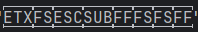
\includegraphics{img}\\
\text{Given:}
\[ F'(k, x\|y) = F(k, 0\|x) \oplus F(k, y\|1) \]
where \( x, y \in \{0, 1\}^{n-1} \).
Let's consider a counter-example:
If the adversary selects \( x = 1^{n-1} \) (all 1s) and \( y = 0^{n-1} \) (all 0s), then the following occurs:
\[ F'(k, x\|y) = F(k, 01^{n-1}) \oplus F(k, 0^{n-1}1) \]
The left component becomes:
\[ F(k, 01^{n-1}) \]
And the right component becomes:
\[ F(k, 0^{n-1}1) \]
Given the bitwise XOR operation, the beginning element will be \( 1 \oplus 1 = 0 \) and the last element will be \( 1 \oplus 1 = 0 \).
All other elements for both \( x \) and \( y \) remain the same, which means they will also be zero.
Thus, the function will produce only zeros, making it distinguishable from a random function.
Hence, \( F' \) does not satisfy the definition of a pseudo-random function when given this adversary's choice.



\begin{verbatim}
[3.1] Using F'(k, m) = F(k, m)||0^n
[3.1] Message: THEWAND
[3.1] Key: MAGIC
[3.1] Result: FHKECZD0000000
[3.2] Using F'(k, m1||m2) = F(k, m1)||F(k, m2 ⊕ 0^n)
[3.2] Message 1: THEWAND
[3.2] Message 2: CHOOSER
[3.2] Key: MAGIC
[3.2] Result: FHKECZDLFHBL
[3.3] Using F'(k, m1||m2) = F(k, 0||m1) ⊕ F(k, m2||1)
[3.3] Message 1: THEWAND
[3.3] Message 2: CHOOSER
[3.3] Key: MAGIC
[3.3] Result: 
\end{verbatim}

Proof can be seen in code: \href{https://stackblitz.com/edit/js-ekqepc?devtoolsheight=80&file=hw23.js&hideDevTools=false}{\texttt{stackblitz hw23}}\\
Code is also in repository: \href{https://github.com/Nurech/js-ekqepc}{\texttt{here}}

\section{Task}%4

\subsection*{4.1: Encryption using Permutation Cipher in OFB Mode}

Given:
\begin{align*}
  D &= 00011 \\
  O &= 01110 \\
  G &= 00110 \\
\end{align*}

Thus, the plaintext in binary is:
\[
  P = 00011\,01110\,00110
\]

For the OFB mode with key \( K = (4,1,3,5,2) \):

\begin{align*}
  1. &\text{ IV } w = 01011 \rightarrow \text{Permute to get } 10011 \\
  2. &\text{ XOR } P_1 \text{ with IV to get } C_1: 00011 \oplus 10011 = 10000 \\
  3. &\text{ Continue for } P_2, P_3 \text{ to get } C_2, C_3
\end{align*}

Resulting in:
\[
  C = 10000\,10100\,11111
\]

\subsection*{4.2: Decryption with Modified Ciphertext}

Flipping the 5-th bit of \( C \):
\[
  C' = 10001\,10100\,11111
\]
Decryption yields:
\[
  P' = 00010\,01110\,00110
\]
Differing from \( P \) by 1 bit.

\subsection*{4.3: Decryption with Modified IV}

Using the modified IV \( w' = 11011 \), decryption provides:
\[
  P'' = 01011\,01111\,00100
\]
This differs from \( P \) by 3 bits.\\

\begin{verbatim}
[4] Binary Plaintext D: 00011 O: 01110 G: 00110
[4] After Permutation (using key): 10011
[4] XOR of Plaintext block: 00011 with iv: 10011 and get EncBlock: 10000
[4] After Permutation (using key): 11010
[4] XOR of Plaintext block: 01110 with iv: 11010 and get EncBlock: 10100
[4] After Permutation (using key): 11001
[4] XOR of Plaintext block: 00110 with iv: 11001 and get EncBlock: 11111
[4.1] Encrypted Ciphertext: 10000 10100 11111
[4.2] Modified Ciphertext by flipping 5-th bit: 100011010011111
[4.2] Decrypted Binary for modified Ciphertext: 000100111000110
[4.2] originalBinaryPlaintext: 000110111000110
[4.2] decryptedBinary2: 000100111000110
[4.2] changedBits2: 1
[4.3] Decrypted Binary using modified IV: 010110111100100
[4.3] decryptedBinary3: 010110111100100
[4.3] originalBinaryPlaintext: 000110111000110
[4.3] Number of bits changed in plaintext for: 3
\end{verbatim}

Proof can be seen in code: \href{https://stackblitz.com/edit/js-ekqepc?devtoolsheight=80&file=hw2_4.js&hideDevTools=false}{\texttt{stackblitz hw24}}\\
Code is also in repository: \href{https://github.com/Nurech/js-ekqepc}{\texttt{here}}

\section{Task}%5

\documentclass{article}
\usepackage{tikz}
\usetikzlibrary{positioning}

\begin{document}
  \section{Task}

  \begin{tikzpicture}
    % Nodes
    \node (iv) {IV: $r_0$};
    \node [below of=iv, node distance=2cm] (m1) {$m_1$};
    \node [below of=m1, node distance=2cm] (m2) {$m_2$};
    \node [below of=m2, node distance=2cm] (mn) {$m_n$};
    \node [right of=iv, node distance=3cm] (e1) {$E(k, m_1)$};
    \node [below of=e1, node distance=2cm] (e2) {$E(k, m_2)$};
    \node [below of=e2, node distance=2cm] (en) {$E(k, m_n)$};
    \node [right of=e1, node distance=3cm] (c1) {$c_1$};
    \node [below of=c1, node distance=2cm] (c2) {$c_2$};
    \node [below of=c2, node distance=2cm] (cn) {$c_n$};

    % Paths
    \path [->] (iv) edge (e1);
    \path [->] (m1) edge (e1);
    \path [->] (m2) edge (e2);
    \path [->] (mn) edge (en);
    \path [->] (e1) edge node[above] {$\oplus$} (c1);
    \path [->] (c1) edge (e2);
    \path [->] (e2) edge node[above] {$\oplus$} (c2);
    \path [->] (c2) edge (en);
    \path [->] (en) edge node[above] {$\oplus$} (cn);
  \end{tikzpicture}

  \subsection*{Decryption Process}

  XOR is its own inverse, so the decryption process is almost identical to the encryption process but in reverse order.
  To decrypt you would do the following:

  \begin{tikzpicture}
    % Nodes
    \node (iv) {IV: $r_0$};
    \node [below of=iv, node distance=2cm] (c1) {$c_1$};
    \node [below of=c1, node distance=2cm] (c2) {$c_2$};
    \node [below of=c2, node distance=2cm] (cn) {$c_n$};
    \node [right of=iv, node distance=3cm] (d1) {$D(k, c_1)$};
    \node [below of=d1, node distance=2cm] (d2) {$D(k, c_2)$};
    \node [below of=d2, node distance=2cm] (dn) {$D(k, c_n)$};
    \node [right of=d1, node distance=3cm] (m1) {$m_1$};
    \node [below of=m1, node distance=2cm] (m2) {$m_2$};
    \node [below of=m2, node distance=2cm] (mn) {$m_n$};

    % Paths
    \path [->] (iv) edge (d1);
    \path [->] (c1) edge (d1);
    \path [->] (c2) edge (d2);
    \path [->] (cn) edge (dn);
    \path [->] (d1) edge node[above] {$\oplus$} (m1);
    \path [->] (m1) edge (d2);
    \path [->] (d2) edge node[above] {$\oplus$} (m2);
    \path [->] (m2) edge (dn);
    \path [->] (dn) edge node[above] {$\oplus$} (mn);
  \end{tikzpicture}




\section{Task}%6

\subsection*{6.1: Output each integer five times}
Given that one output operation takes a constant amount of time (let's call this constant \(c\)), for \(n\) integers, outputting each 5 times will take \(5nc\) time.

\begin{align*}
  \text{Time for 1} & : 5nc = c \times O(n) = O(5 \times n)
\end{align*}

\subsection*{6.2: Apply bubble sort}
In bubble sort, we repeatedly traverse the array and swap adjacent elements if they are in the wrong order. The worst-case occurs when the array is reverse sorted, which requires \(\frac{n(n-1)}{2}\) comparisons and swaps.
Let's take a simple reversed array of size 4 for illustration: \( \{4, 3, 2, 1\} \)

\begin{itemize}
  \item \textbf{1\textsuperscript{st} pass}: Compare 4 and 3, 3 and 2, 2 and 1. 3 swaps. Array becomes \( \{3, 2, 1, 4\} \)
  \item \textbf{2\textsuperscript{nd} pass}: Compare 3 and 2, 2 and 1. 2 swaps. Array becomes \( \{2, 1, 3, 4\} \)
  \item \textbf{3\textsuperscript{rd} pass}: Compare 2 and 1. 1 swap. Array becomes \( \{1, 2, 3, 4\} \)
\end{itemize}

\begin{align*}
  \text{Time for 2} & : \frac{n(n-1)}{2} = O(n^2)
\end{align*}

  \subsection*{6.3: Find the greatest common divisor of the 2\textsuperscript{nd} and 4\textsuperscript{th} elements of the array}

  Accessing specific positions within an array, such as the 2\textsuperscript{nd} and 4\textsuperscript{th} elements, is a direct operation with constant time complexity, denoted as \(O(1)\).
  For the computation of the GCD, the Euclidean algorithm is typically employed.
  The worst-case time complexity of the Euclidean algorithm is bounded by the number of digits in the smaller number.
  Let's denote the time complexity of the algorithm by \(T(a, b)\), where \(a\) and \(b\) are the two numbers with \(a > b\).

  \begin{equation}
    T(a, b) = 1 + T(b, a \mod b)
  \end{equation}

  The equation above illustrates the recursive nature of the Euclidean algorithm.
  The worst-case scenario occurs when every iteration reduces the number by a constant factor.
  This corresponds to the Fibonacci sequence, as demonstrated by \href{https://en.wikipedia.org/wiki/Lam%C3%A9%27s_theorem#Proof}{\texttt{Lamé's theorem}}.
  Given Lamé's theorem, the number of steps required is bounded by the index of the Fibonacci number that is closest to \(b\).
  If this index is \(h\), then:

  \begin{equation}
    F_h \approx \phi^h \Rightarrow h \approx \log_{\phi} b
  \end{equation}

  Where \( \phi \) is the golden ratio.
  Therefore, the time complexity can be expressed in terms of the logarithm:

  \begin{equation}
    \text{Time for Step 3} : O(\log b)
  \end{equation}

  In essence, the \(O(\log b)\) complexity arises because the number of divisions required by the Euclidean algorithm is at
  most proportional to the number of digits in \(b\), which scales logarithmically with \(b\).



\section{Task Bonus}

  Consider the security games as shown in Figure 1. The encryption scheme can be considered secure if
  \[ \Pr[b = 1 : \text{Game 0}] - \Pr[b = 1 : \text{Game 1}] \leq \varepsilon \]
  where \( \varepsilon \) is negligible. This means that no adversary should be able to differentiate between the two games based on the encryption of messages \( m_0 \) and \( m_1 \).

  However, let's consider the following attack:

  \begin{enumerate}
    \item The adversary prepares two messages, \( m_0 \) and \( m_1 \), both two blocks in length.
    \item These messages are sent to the challenger.
    \item The challenger generates a one-block long key using \( k \leftarrow \text{KeyGen()} \).
    \item The challenger also generates a random initialization vector (IV).
    \item The challenger randomly chooses between the two messages, \( m_0 \) or \( m_1 \), to encrypt.
    \item Using the selected key and IV, the challenger encrypts the chosen message in CBC mode.
    \item The resulting ciphertext along with the IV is then sent back to the adversary.
  \end{enumerate}

  In this scenario, when the OTP is used in CBC mode, the adversary can exploit the chaining property.
  Specifically, if the adversary knows a block of plaintext and its corresponding ciphertext, information about the subsequent plaintext block can be inferred.
  Given that the adversary prepared the messages and knows their content, they can attempt to decrypt the received ciphertext using the IV and the known plaintext block.
  If the decryption matches one of the prepared messages, the adversary can determine which message was encrypted by the challenger.
  This breaks the security definition, as the adversary can now differentiate between Game 0 and Game 1, making the difference in probabilities larger than the negligible \( \varepsilon \).
  Therefore, the OTP in CBC mode fails to meet the security definition as presented in the security games.

  Let's consider two messages \( m_0 \) and \( m_1 \) that are both two blocks in length:
  \begin{align*}
    m_0 &= [P_0, P_1] \\
    m_1 &= [P_2, P_3]
  \end{align*}

  When encrypting using CBC mode with OTP, the encryption for a block can be represented as:
  \[ C_i = P_i \oplus C_{i-1} \]
  where \( C_{i-1} \) is the ciphertext of the previous block and \( \oplus \) denotes the XOR operation.

  Given a random Initialization Vector (IV), the encryption of the first block is:
  \[ C_0 = P_0 \oplus \text{IV} \]
  for \( m_0 \) and:
  \[ C_0' = P_2 \oplus \text{IV} \]
  for \( m_1 \).

  Now, for the second block:
  \[ C_1 = P_1 \oplus C_0 \]
  for \( m_0 \) and:
  \[ C_1' = P_3 \oplus C_0' \]
  for \( m_1 \).

  If an adversary knows \( P_0 \) and \( C_0 \), they can compute:
  \[ P_1 \oplus C_1 = P_1 \oplus (P_1 \oplus C_0) = C_0 \]
  Similarly, for \( m_1 \):
  \[ P_3 \oplus C_1' = P_3 \oplus (P_3 \oplus C_0') = C_0' \]

  Hence, by observing the ciphertexts, the adversary can distinguish between the encryptions of \( m_0 \) and \( m_1 \) based on the derived values of \( C_0 \) and \( C_0' \), thus breaking the security definition.


\end{document}
